\section{Electromagnetismo}

\subsection{Introducción}

El imán es un cuerpo o dispositivo con un magnetismo significativo, de forma que atrae a otros imanes o metales ferromagnéticos (por ejemplo, hierro, cobalto, níquel y aleaciones de estos). El magnetismo es el conjunto de fenómenos físicos mediados por campos magnéticos, que son una representación matemática del modo en que las fuerzas magnéticas interactúan y se distribuyen en el espacio.

\begin{figure}[ht]
  \centering
  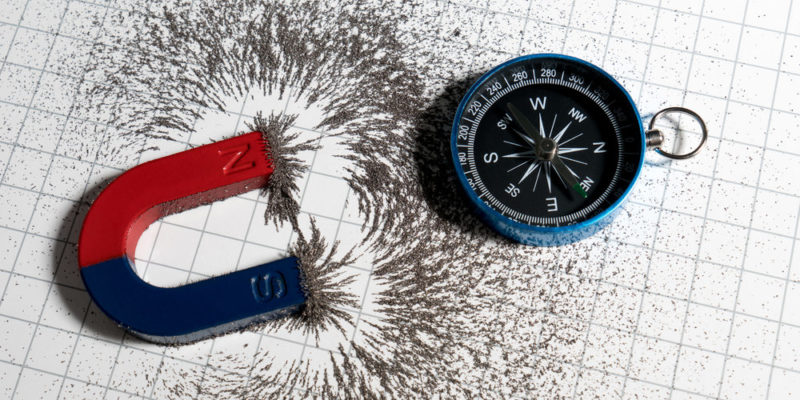
\includegraphics[width=0.5\textwidth]{iman-brujula.jpg}
  \caption{Limaduras de hierro y brújula afectados por un imán de herradura}
  \label{fig:iman}
\end{figure}

Como se puede apreciar en la figura \ref{fig:iman}, todos los imanes poseen dos polos, llamados \textit{polo norte} y \textit{polo sur}. Cualquiera de los polos de un imán atrae a un objeto ferromagnético no magnetizado, y, al igual que pasaba con las cargas eléctricas, los polos iguales se repelen y los polos opuestos se atraen. Es decir polo norte y polo sur se atraen, mientras que polo norte y polo norte (o sur y sur) se repelen.

La relación entre la electricidad y el magnetismo fue descubierta en 1819, cuando en el transcurso de una demostración en una conferencia, el científico danés Hans Christian Oersted descubrió que una corriente eléctrica en un alambre desviaba la aguja de una brújula cercana. Durante 1820, Faraday y Joseph Henry demostraron, de manera independiente relaciones adicionales entre la electricidad y el magnetismo. Mostraron que es posible crear una corriente eléctrica en un circuito ya sea moviendo un imán cerca de él o variando la corriente de algún circuito cercano. Estas observaciones demuestran que una variación en un campo magnético crea un campo eléctrico. Años después, el trabajo teórico de Maxwell demostró que lo contrario también es cierto: un campo eléctrico que varía crea un campo magnético.

\subsection{Magnetismo}

Tal vez el concepto de polos magnéticos parezca similar al de carga eléctrica, y los polos norte y sur parezcan análogos a las cargas positiva y negativa. No obstante, tal analogía puede ser errónea. Si bien las cargas positiva y negativa existen aisladas, no hay evidencia experimental de que exista un polo magnético aislado.

Los imanes siempre se encuentran como dipolos magnéticos (norte y sur), y no se ha comprobado la existencia los monopolos magnéticos.

\subsubsection{Campo Magnético}

Al igual que el campo eléctrico, el magnético es un \hl{\textit{campo vectorial}}, es decir, una cantidad vectorial asociada con cada punto del espacio. La existencia de un campo magnético en algún punto del espacio puede determinarse midiendo la magnitud de la \textbf{fuerza magnética} que ejerce el campo sobre una partícula de prueba ubicada en ese punto.

En esencia el magnetismo es un fenómeno físico asociado al movimiento de cargas eléctricas, que da lugar a fuerzas de atracción o repulsión entre materiales. Se manifiesta principalmente a través de los campos magnéticos, los cuales son representaciones vectoriales que describen la influencia que una corriente eléctrica o un material magnético ejerce en su entorno.

Desde un punto de vista fundamental, \hl{el origen del magnetismo reside en el movimiento de cargas eléctricas} a nivel microscópico, particularmente en el espín y el momento orbital de los electrones en los átomos. En materiales como el hierro, cobalto y níquel, estos momentos magnéticos atómicos se alinean de manera colectiva, generando imanes permanentes.

El \textbf{campo magnético} se representa mediante el vector \(\vec{B}\), cuya unidad en el Sistema Internacional es el tesla (T)\footnote{Un tesla equivale a: \(T \equiv \frac{Ns}{Cm} \equiv \frac{N}{Am}\)}. La interacción de una carga en \textbf{movimiento} \(q\) con un campo magnético está regida por la fuerza magnética, expresada como:
\begin{equation}
  \vec{F}_B = q\vec{v} \times \vec{B}
  \label{eq:fuerza_magnética}
\end{equation}
donde \(\vec{v}\) es el vector velocidad de la partícula. Esta fuerza es perpendicular tanto a la dirección de la velocidad como a la del campo magnético.

\begin{figure}[ht]
  \centering
  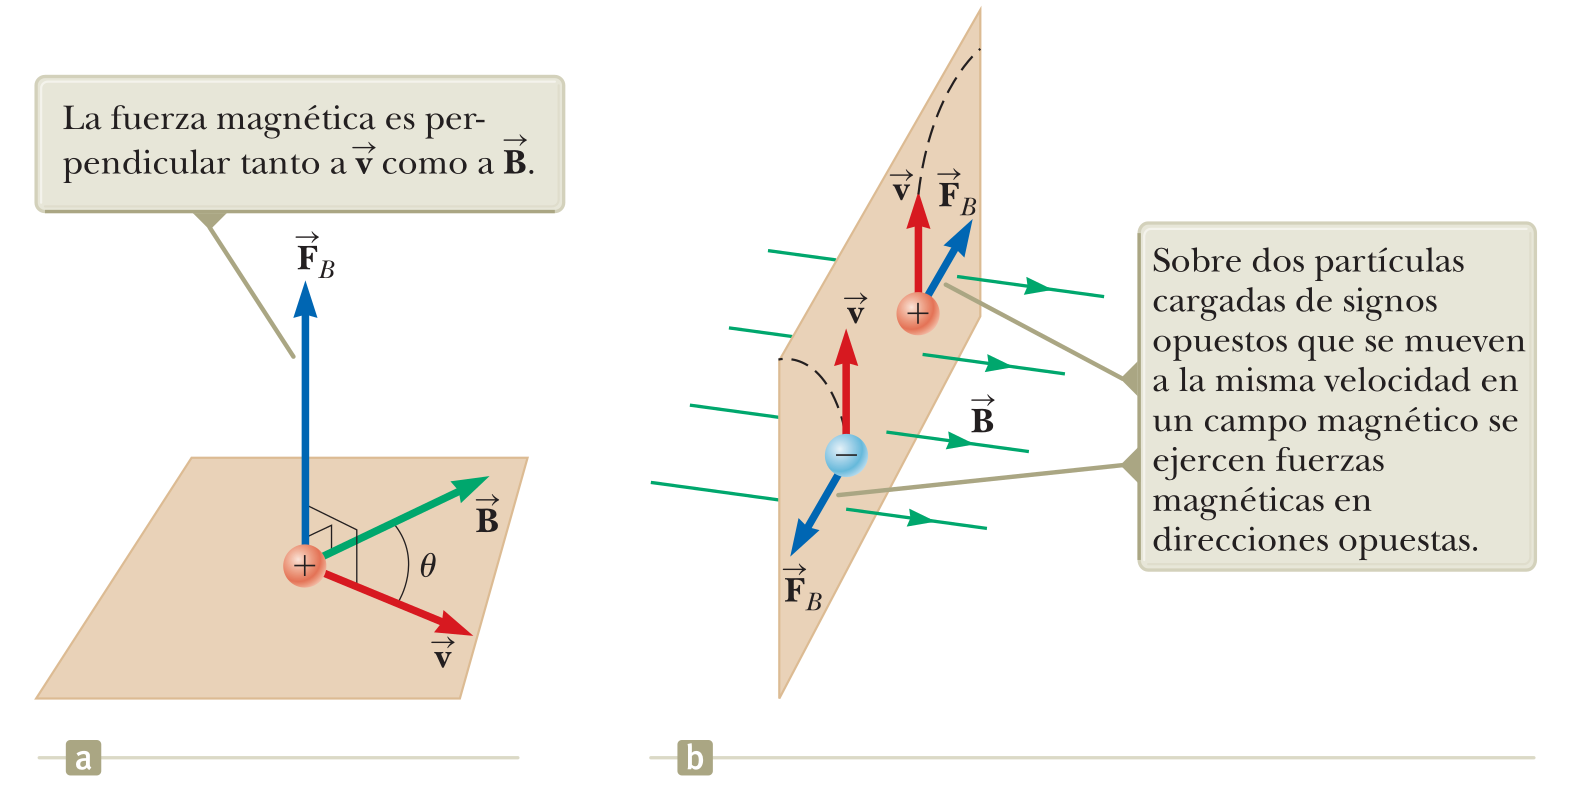
\includegraphics[width=0.8\textwidth]{magnetic_force.png}
  \caption{Partículas con carga atravesando un campo magnético \(\vec{B}\) con una velocidad \(\vec{v}\)}
\end{figure}

Si se conoce el ángulo \(\theta\) entre el vector velocidad \(\vec{v}\) y el campo magnético \(\vec{B}\) la fuerza se puede calcular como:
\[
  \vec{F}_B = \left\lvert q \right\rvert v B \sin(\theta) \hat{r}
\]
donde \(\hat{r}\) es un versor\footnote{versor: vector de módulo 1} normal al plano formado por los vectores \(\vec{v}\) y \(\vec{B}\). 

Comparando la fuerza magnética con la fuerza eléctrica se puede ver que la fuerza \(\vec{F}_B\) es perpendicular al campo magnético y a la velocidad de la partícula, mientras que \(\vec{F}_e\) se ejerce sobre la dirección del campo eléctrico. Además \(\vec{F}_e\) no requiere que la partícula con carga esté en movimiento.

\subsubsection{Lineas de campo magnético}

\begin{wrapfigure}{r}{0.3\textwidth}
  \centering
  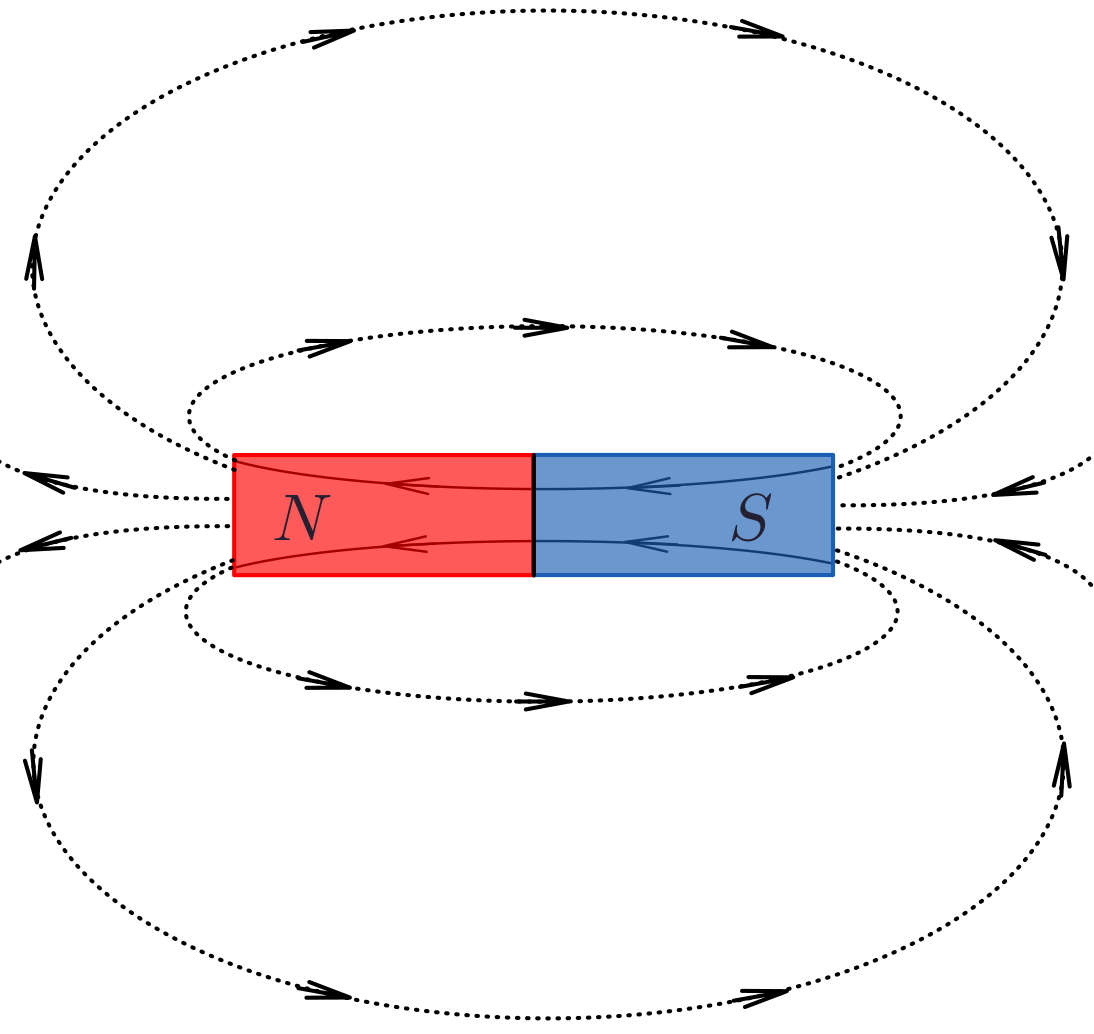
\includegraphics[width=\linewidth]{magnetic_field_lines.png}
  \caption{Líneas de campo magnético.}
  \label{fig:lineas_de_iman}
\end{wrapfigure}
La representación de los campos magnéticos mediante líneas de campo magnético es muy útil para visualizar la intensidad y la dirección del campo magnético. Como se muestra en la figura \ref{fig:lineas_de_iman}, cada una de estas líneas forma un bucle cerrado, aunque no se muestren todas las líneas cerradas por las limitaciones del espacio disponible puede observarse en las líneas de campo más cercanas al cuerpo del imán que salen del polo norte (\(N\)), hacen un bucle hacia el polo sur (\(S\)) y continúan a través de la barra magnética de vuelta al polo norte. Dentro del imán las líneas están muy juntas, pero nunca se cortan o tocan entre sí.

Las líneas de campo magnético tienen varias reglas estrictas:
\begin{enumerate}
  \item La dirección del campo magnético \(\vec{B}\) es tangente a la línea de campo en cualquier punto del espacio. Una pequeña brújula señalará la dirección de la línea del campo.
  \item La fuerza del campo es proporcional a la cercanía de las líneas. Es exactamente proporcional al número de líneas por unidad de superficie perpendicular a las líneas (llamada densidad de área). Es el mismo concepto que en las líneas de campo eléctrico. Mientras más juntas están mayor intensidad tiene.
  \item Las líneas de campo magnético no pueden cruzarse nunca, lo que significa que el campo es único en cualquier punto del espacio.
  \item Las líneas de campo magnético son continuas, formando bucles cerrados sin principio ni fin. Se dirigen del polo norte al polo sur.
\end{enumerate}

La última propiedad está relacionada con el hecho de que los polos norte y sur no pueden separarse. Es una diferencia clara respecto a las líneas de campo eléctrico, que generalmente comienzan en cargas positivas y terminan en cargas negativas o en el infinito. Si existieran cargas magnéticas aisladas (denominadas monopolos magnéticos), las líneas de campo magnético comenzarían y terminarían en ellas. Puedes ver más ejemplos sobre líneas de campo magnético en \href{https://openstax.org/books/f%C3%ADsica-universitaria-volumen-2/pages/11-2-campos-y-lineas-magneticas}{OpenStax} (\cite{openstax})

\begin{figure}[ht]
  \centering
  \begin{subfigure}[b]{0.35\textwidth}
      \centering
      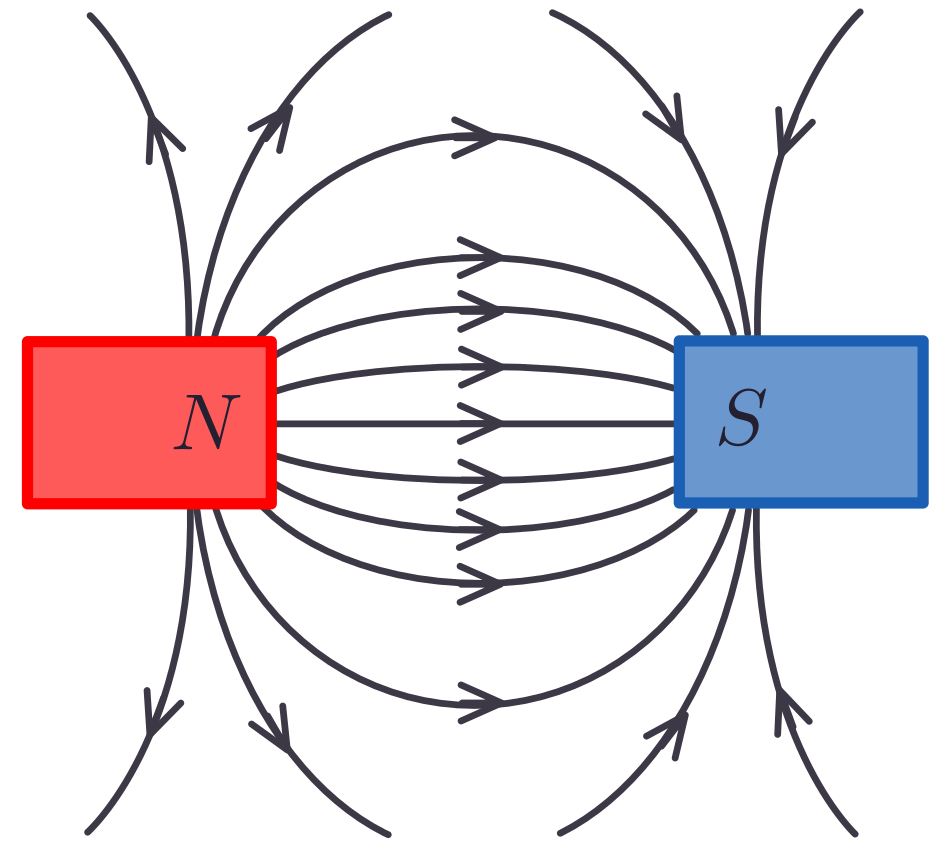
\includegraphics[width=\textwidth]{magnetic_lines_a.png}
      \caption{Líneas de campo magnético entre polos opuestos.}
      \label{fig:polos_opuestos}
  \end{subfigure}
  \hspace{10pt}
  \begin{subfigure}[b]{0.35\textwidth}
      \centering
      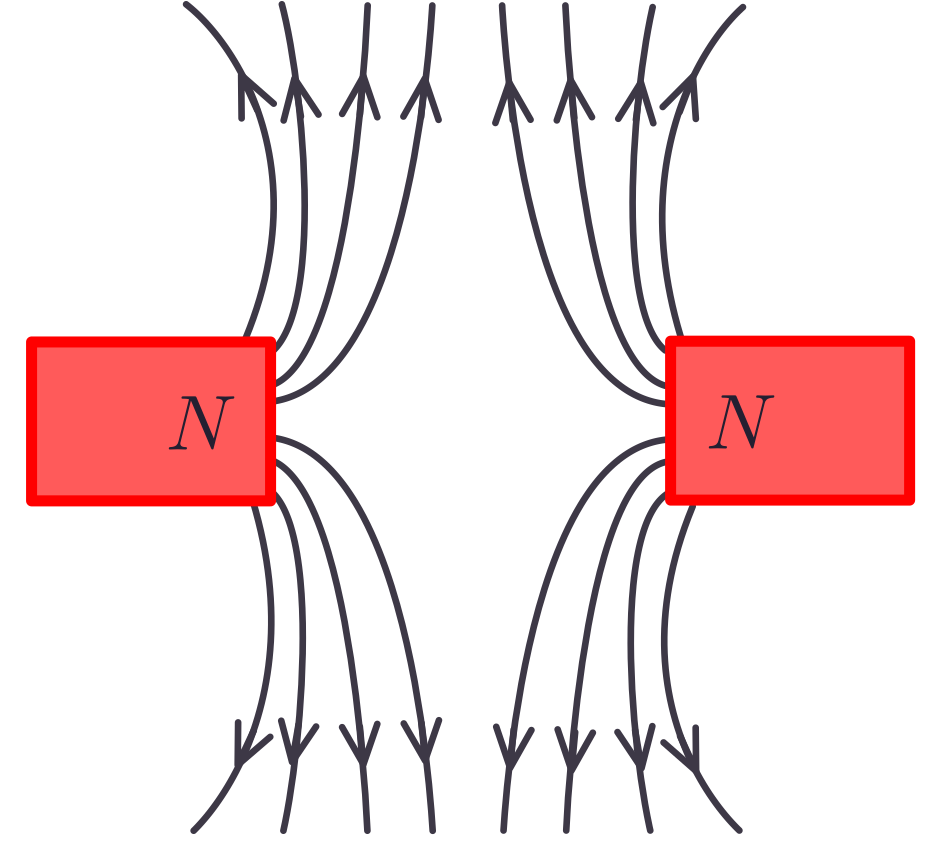
\includegraphics[width=\textwidth]{magnetic_lines_b.png}
      \caption{Líneas de campo magnético entre polos similares.}
      \label{fig:polos_iguales}
  \end{subfigure}
  \caption{Lineas de campo para distintas configuraciones de imanes.}
  \label{fig:lineas_de_campo_magnético_entre_imanes}
\end{figure}

Como se puede observar en la figura \ref{fig:lineas_de_campo_magnético_entre_imanes} las líneas de campo magnético se definen para tener la dirección en la que apunta una pequeña brújula cuando se coloca en un lugar del campo. La fuerza del campo es proporcional a la cercanía (o densidad) de las líneas. Si se pudiera sondear el interior del imán, se encontraría que las líneas de campo forman bucles continuos y cerrados. Para ajustarse a un espacio razonable, algunos de estos dibujos pueden no mostrar el cierre de los bucles; sin embargo, si se dispusiera de espacio suficiente, los bucles estarían cerrados. 

Nótese que en la figura \ref{fig:polos_opuestos} el campo que se forma en el centro de los imanes es casi uniforme. Este concepto es útil ya que este tipo de campo se encuentra en los imanes de herradura (como el que está en la figura \ref{fig:iman}). Por otro lado en la figura \ref{fig:polos_iguales} el campo entre imanes es casi cero (muy poca intensidad) ya que las líneas de campo magnético están muy separadas entre sí.

\subsubsection{Flujo Magnético}
\label{sec:flujo_magnético}

Definimos el \textbf{flujo magnético} \(\Phi_B\) a través de una superficie igual que definimos el flujo eléctrico en relación con la ley de Gauss en la sección \ref{sec:flujo_electrico}. 

El flujo magnético es una magnitud escalar que cuantifica la cantidad de campo magnético que atraviesa una superficie dada. Matemáticamente, se define como la integral del producto escalar entre el campo magnético \(\vec{B}\) y el vector diferencial de área \(d\vec{A}\) de la superficie:

\[
\Phi_B = \int_S \vec{B} \cdot d\vec{A}
\]
donde:
\begin{itemize}
  \item \(\Phi_B\) es el flujo magnético,
  \item \(S\) es la superficie sobre la que se calcula el flujo,
  \item \(\vec{B}\) es el vector del campo magnético,
  \item \(d\vec{A}\) es un elemento diferencial de área, cuyo módulo es el área diferencial y cuya dirección es perpendicular a la superficie, siguiendo la convención del sentido positivo (normal saliente en una superficie cerrada).
\end{itemize}

Al igual que el flujo eléctrico, el flujo magnético mide cuántas ``líneas de campo magnético'' atraviesan una superficie. Si el campo es perpendicular a la superficie, el flujo es máximo; si es paralelo, el flujo es nulo.

En el caso especial donde el campo magnético es uniforme y la superficie es plana, la expresión se simplifica a:
\[
\Phi_B = B A \cos\theta
\]
donde:
\begin{itemize}
  \item \(B\) es la magnitud del campo magnético,
  \item \(A\) es el área de la superficie,
  \item \(\theta\) es el ángulo entre el vector \(\vec{B}\) y el vector normal a la superficie.
\end{itemize}

La unidad de flujo magnético en el Sistema Internacional es el weber (Wb), donde: \(1 \, \text{Wb} = 1 \, \text{T} \cdot \text{m}^2\)

Si recuerda el \textit{flujo eléctrico} y la ley de Gauss de la sección \ref{sec:ley_de_gauss} podríamos intuir que para el magnetismo pasa algo similar. Sin embargo como no existen los monopolos magnéticos y las líneas de campo magnético son cerradas \hl{el flujo magnético sobre una superficie cerrada es siempre cero.}
\[
\oint \vec{B}\cdot d\vec{A} = 0
\]
Digamos, en palabras simples: si encerramos un imán en una superficie Gaussiana, todas las líneas de campo magnético que salen, vuelven a entrar. Esto resulta en un flujo nulo.

\subsubsection{Trabajo del campo magnético}

En la sección \ref{sec:potencial} vimos como una carga que se mueve en un campo eléctrico realiza un trabajo. En esta sección las partículas deben estar si o si en movimiento para verse afectadas por el campo magnético. Entonces ¿Será que están realizando trabajo? La respuesta rápida es que no. Veamos el por qué: recordando que el trabajo es el \textbf{producto escalar} entre la fuerza por la distancia (o desplazamiento), si la fuerza es perpendicular al desplazamiento entonces dará siempre cero.
En base a esto, vemos que \(\vec{F}_B\) no realiza trabajo ni cambia la energía del sistema carga-campo por ser perpendicular al plano de \(\vec{B}\) y \(\vec{v}\). 

\begin{tcolorbox}[myconclusion]
  Con base en este último enunciado y también con el teorema trabajo-energía cinética, se concluye que la energía cinética de una partícula cargada que se mueve a través de un campo magnético \textbf{no} puede ser modificada sólo por el campo magnético. El campo magnético puede modificar la dirección del vector velocidad, pero no puede cambiar la rapidez ni la energía cinética de la partícula.
\end{tcolorbox}

\begin{wrapfigure}{l}{0.3\textwidth}
  \centering
  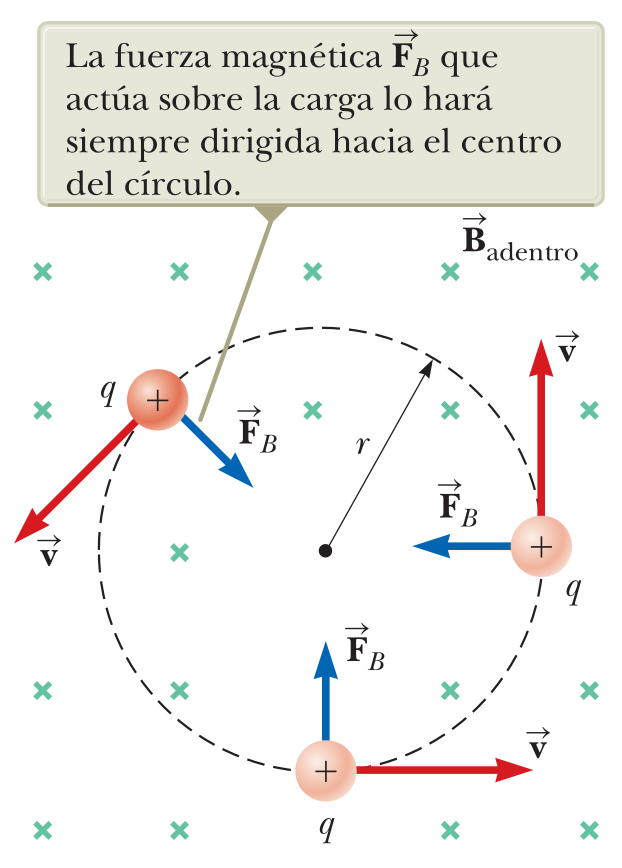
\includegraphics[width=\linewidth]{centipet_force.png}
  \caption{Fuerza magnética para una partícula con velocidad \(v\) y un campo magnético entrante.}
  \label{fig:centripet_force}
\end{wrapfigure}
\subparagraph{Pregunta:}

\noindent ¿Qué tipo de fuerza es siempre perpendicular a la trayectoria de una partícula y no modifica la magnitud de la velocidad?

\vspace{3pt}

\noindent La \textbf{fuerza centrípeta}. Entonces, la fuerza magnética, como se ve en la figura \ref{fig:centripet_force} es una fuerza centrípeta para una partícula cargada y en movimiento. Por lo tanto podemos ocupar todas las ecuaciones del movimiento circular.

Si no recuerdas bien los temas de dinámica y las ecuaciones del movimiento circular uniforme y no uniforme puedes volver a verlo en la sección \ref{sec:mcu}

Con este principio, se observa que para la situación ilustrada en la figura \ref{fig:centripet_force} la magnitud de \(\vec{F}_B\) y \(\vec{v}\) son constantes. Como \(\vec{F}_B \equiv \vec{F}_c\) entonces podemos igualar \(\vec{F}_B\) a la expresión de aceleración centrípeta:
\[
  F_B = qvB = m \frac{v^2}{r}
\]
\clearpage

\subsection{Fuerza de Lorentz}

Una carga móvil con una velocidad \(\vec{v}\), en presencia tanto de un campo eléctrico \(\vec{E}\) como de un campo magnético \(\vec{B}\) es descrito por dos modelos de partícula en un campo. Experimenta a la vez una fuerza eléctrica \(\vec{F}_E=q\vec{E}\) y una fuerza magnética \(\vec{F}_B=q\vec{v} \times \vec{B}\). La fuerza total es la fuerza de Lorentz:

\begin{equation}
  \vec{F} = q\left(\vec{E} + \vec{v} \times \vec{B}\right)
  \label{eq:f_lorentz}
\end{equation}

\subsubsection{Fuerza magnética en un conductor}
\label{sec:fuerza_magnetica_en_un_conductor}

\begin{wrapfigure}{r}{0.3\textwidth}
  \centering
  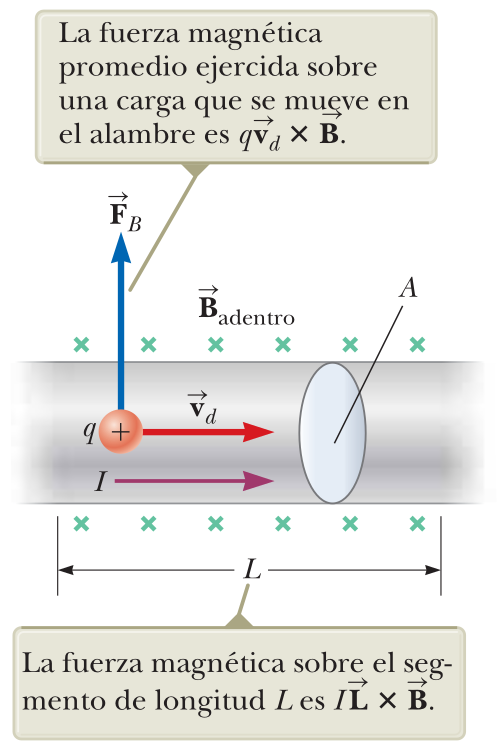
\includegraphics[width=0.3\textwidth]{lorentz.png}
  \caption{Un segmento de un alambre conduciendo corriente en un campo magnético \(\vec{B}\)}
  \label{fig:lorentz}
\end{wrapfigure}
Ahora hagamos un análisis de las fuerzas que interactúan para un cable conductor como el que se muestra en la figura \ref{fig:lorentz}. Vemos que en la figura el campo magnético es entrante. Si no circula corriente eléctrica, entonces no hay movimiento de cargas, por ende las cargas tendrán una \(v_d=0\) y la fuerza magnética será cero. Si hacemos circular cargas sobre el conductor aplicando una diferencia de potencial entre las puntas del conductor, entonces \(v_d \neq 0\) y por lo tanto existirá una fuerza magnética. 
Conviene cuantificar esta explicación considerando la longitud \(L\) del segmento y el área de sección transversal \(A\). Al tener en cuenta las dimensiones del cable, podemos expresar la \textbf{fuerza total} que sentirá el cable. Sabiendo que la corriente que circula por el cable es \(I = nq v_d A\) y el volumen del cable es \(AL\) entonces: 
\[
  \vec{F}_B = (q\vec{v}_d \times \vec{B})nAL
\]
Reemplazando \(I=qn \vec{v}_d A\) en la expresión:
\[
  \vec{F}_B = I\vec{L} \times \vec{B}
\]
donde \(\vec{L}\) es un vector que apunta en la dirección de la corriente \(I\) y tiene una magnitud igual a la longitud \(L\). Si se expresa el producto vectorial como el módulo de los vectores por el seno del ángulo entre ellos:
\begin{equation}
  \boxed{F_B = IL \cdot B \, \sin(\theta)}
  \label{eq:fuerza_magnetica_en_un_conductor}
\end{equation}

\subsection{Momento de torsión sobre una espira}

Es importante que antes de abordar esta sección se haya entendido bien la sección anterior (\ref{sec:fuerza_magnetica_en_un_conductor}) y que recuerde qué es torque. Si desea ver un recordatorio sobre torque puede utilizar el resumen dado en la sección \ref{sec:torque_y_momento_de_inercia}.

\subsubsection{Definición de espira}

Tal vez parezca trivial definir el concepto de espira, sin embargo vamos a aclarar los elementos que vamos a usar para demostrar cómo generamos el par de torsión. Entonces, una espira es un lazo de alambre por el que puede fluir corriente eléctrica. Vamos a tomar una espira rectangular, y vamos a suponer que fluye una corriente como se muestra en la figura \ref{fig:espira_vista_superior}. En este caso estamos ignorando de dónde proviene la corriente eléctrica, y suponiendo que la espira es totalmente cerrada.
\begin{wrapfigure}{l}{0.3\textwidth}
  \centering
  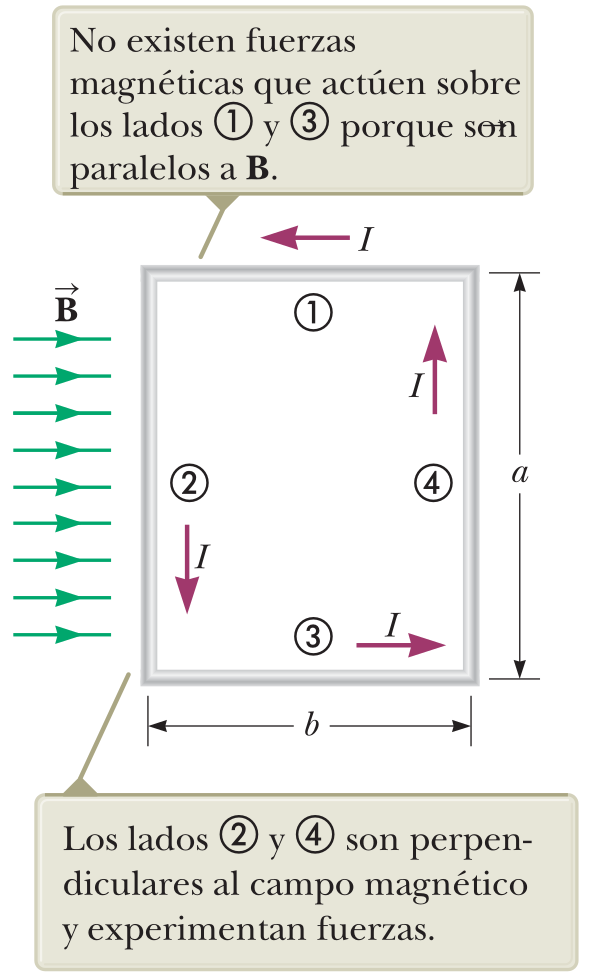
\includegraphics[width=\linewidth]{espira_sup.png}
  \caption{Vista superior de una espira rectangular}
  \label{fig:espira_vista_superior}
\end{wrapfigure}

Cuando la corriente pasa a través de la espira, las cargas fluyen a través del conductor (de la misma forma que vimos en la sección anterior). Si se coloca en un campo magnético uniforme \(\vec{B}\) de modo que sea perpendicular a dos de los segmentos (el segmento \textcircled{2} y \textcircled{4} en caso de la figura \ref{fig:espira_vista_superior}), cada uno experimenta una fuerza magnética dada por la ecuación \eqref{eq:fuerza_magnetica_en_un_conductor} mientras que en los segmentos \textcircled{1} y \textcircled{3} la fuerza magnética será nula ya que el vector \(\vec{v}_d\) y \(\vec{B}\) son paralelos. 

Las fuerzas que actúan sobre los segmentos \textcircled{2} y \textcircled{4} no se cancelan completamente en su efecto mecánico: aunque su suma vectorial puede ser nula (es decir, no producen una traslación neta de la espira), sí generan un momento de torsión o torque que tiende a rotarla.

Entonces, teniendo en cuenta que la longitud de los segmentos \textcircled{2} y \textcircled{4} es \(L=a\), el módulo de la fuerza que siente cada segmento será:
\begin{equation}
  F_{2} = F_{4} = IaB
  \label{eq:fuerza_torque_en_una_espira}
\end{equation}

\begin{tcolorbox}[myconclusion]
  Recuerda: Esta fuerza es perpendicular tanto al elemento de corriente como al campo magnético.
\end{tcolorbox}

\subsubsection{Definición de momento de torsión}

\begin{wrapfigure}{l}{0.3\textwidth}
  \centering
  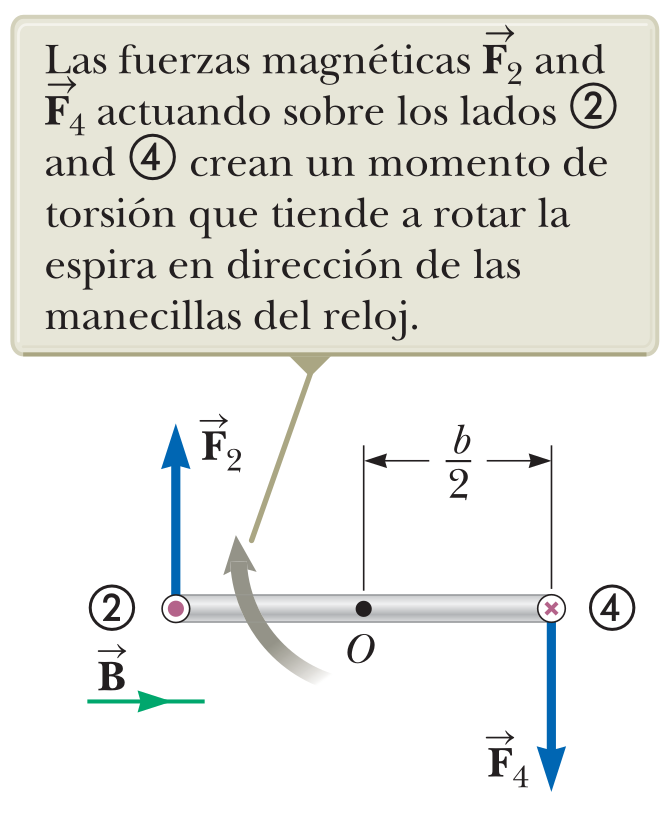
\includegraphics[width=\linewidth]{espira_lat.png}
  \caption{Vista lateral de la espira rectangular}
  \label{fig:espira_vista_lateral}
\end{wrapfigure}
Si analizamos la misma espira de la figura \ref{fig:espira_vista_superior} pero vista desde el lateral para poder visualizar las fuerzas actuantes podemos ver por qué se produce un torque.

Si se aplica la regla de la mano derecha en la figura \ref{fig:espira_vista_superior} podemos ver que en el segmento \textcircled{2} la fuerza es saliente y en el segmento \textcircled{4} la fuerza es entrante. Si vemos la figura \ref{fig:espira_vista_lateral} donde se muestra la misma espira en vista lateral, vemos que sobre el segmento \textcircled{2} la fuerza actúa hacia arriba y sobre el segmento \textcircled{4} actúa hacia abajo. Estas fuerzas no pueden provocar una traslación ya que se cancelan entre sí, pero si pueden provocar una rotación respecto de un eje \(O\).

Sabemos que el módulo del momento de torsión o torque (\(\tau\)) respecto de un eje de giro \(O\) es:
\begin{align*}
  \tau &= F\, r \sin(\theta) \\
  \text{Y}&\,\text{para dos fuerzas actuantes:}\\
  \tau &= \tau_1 + \tau_2 \\
  \tau &= F_1 r_1 \sin(\theta_1) + F_2 r_2 \sin(\theta_2)  
\end{align*}

En nuestra espira, el ángulo \(\theta=\pi/2\) será el mismo para las dos fuerzas \(F_{2}\) y \(F_{4}\), ya que depende del ángulo de la espira con \(\vec{B}\).

En base a esto, entonces observando la figura \ref{fig:espira_vista_lateral} podemos aplicar la expresión de torque a las fuerzas que actúan sobre la espira, resultando:
\begin{align}
  \tau &= F \, r \, \sin(\theta); \quad \text{donde para cada lado: } F=F_B ~~\text{y}~~ r=b/2 \nonumber \\ 
       &= F_{2} \, \frac{b}{2}\, \sin(\theta) + F_{4} \, \frac{b}{2}\, \sin(\theta) \nonumber \\
       &= \left(IaB + IaB\right)\, \frac{b}{2} \, \sin(\theta); \quad \text{donde:}~~ L=a \nonumber \\ 
       &= 2IaB \, \frac{b}{2} \, \sin(\theta) \nonumber \\
       &= IB \, ab \, \sin(\theta); \quad \text{como} ~~ A=ab \nonumber \\
  \tau &= IB \, A \, \sin(\theta)
  \label{eq:torque_para_una_espira}
\end{align}

En este caso como \(\theta = \pi/2\) se obtiene el torque máximo \(\tau_{max} = IAB\), sin embargo la expresión \eqref{eq:torque_para_una_espira} funciona para cualquier ángulo \(\theta\) que forme la espira con respecto a \(\vec{B}\). 

Sabemos que como el torque es definido como producto vectorial entonces \(\tau\) es un vector perpendicular al plano formado por otros dos vectores. En el caso de la espira, como vimos durante el desarrollo \eqref{eq:torque_para_una_espira} sabemos que el campo magnético \(\vec{B}\) es un vector. El otro vector será el área \(\vec{A}\) y, al igual que lo definimos en el flujo eléctrico y magnético, es un vector perpendicular a la superficie. Para comprender mejor el vector área de la espira, puede observarlo en la figura \ref{fig:espira_rotada}

\begin{figure}[ht]
  \centering
  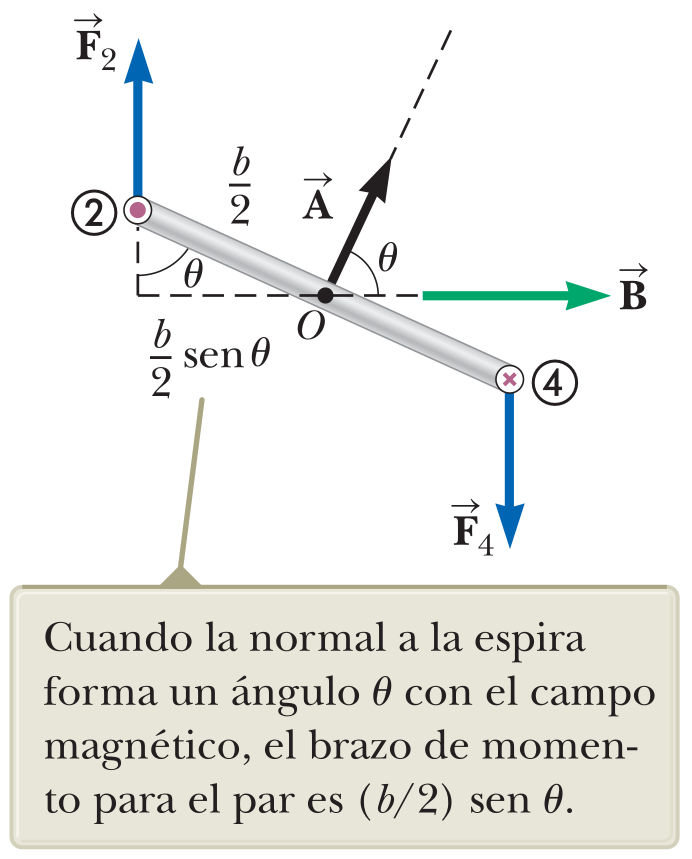
\includegraphics[width=0.4\textwidth]{espira_lat_theta.png}
  \caption{Vista lateral de la espira rectangular rotada un ángulo \(\theta\)}
  \label{fig:espira_rotada}
\end{figure}

En base a esto entonces decimos que \(\vec{tau}\) para una espira es:
\begin{equation}
  \boxed{\vec{\tau} = I\vec{A}\times \vec{B}}
  \label{eq:vec_torque_de_espira}
\end{equation}

Aunque la ecuación \ref{eq:vec_torque_de_espira} se dedujo para una espira rectangular, es válida para una espira plana de cualquier forma.

\subsubsection{Momento dipolar magnético}

El \textbf{momento dipolar magnético} de una \textit{espira} es una \hl{cantidad vectorial} que caracteriza la intensidad y la orientación del campo magnético generado por una corriente eléctrica que circula por una espira cerrada\footnote{En el Sistema Internacional, se mide en \(\text{A·m}^2\) (amperio-metro cuadrado).}.
\[
  \vec{\mu} = I \vec{A}
\]

\begin{wrapfigure}{r}{0.27\textwidth}
  \centering
  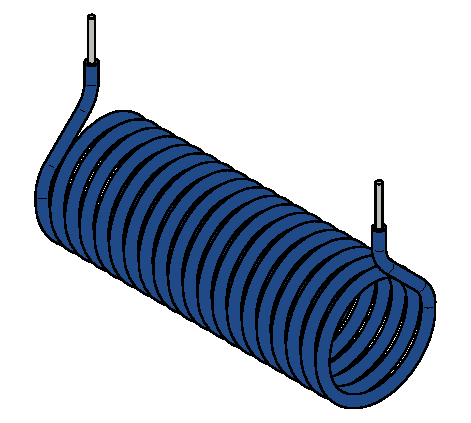
\includegraphics[width=\linewidth]{Solenoid.pdf}
  \caption{Imágen de un solenoide}
  \label{fig:solenoide}
\end{wrapfigure}
Su magnitud está dada por el producto de la corriente eléctrica (\(I\)) que fluye por la espira y el área (\(A\)) encerrada por esta:  
\[
  \mu = I A
\]  
Si se tiene un solenoide de \(N\) vueltas (o espiras), el momento se amplifica:  
\[
  \mu = N I A
\]

\begin{tcolorbox}
  \textbf{Nota}: el término \textit{espira} se suele usar para referirse a un solo lazo de alambre, mientras que un solenoide consiste en múltiples espiras enrolladas en forma de cilindro como se muestra en la figura \ref{fig:solenoide}.
\end{tcolorbox}

\(\vec{A}\) es el vector área de una sola espira o vuelta, su magnitud es el área \(A\) de la espira (por ejemplo en la figura \ref{fig:dipolar_magnet_moment} el área de la espira será \(A=\pi r^2\)), y su dirección es normal al plano de la espira, siguiendo la regla de la mano derecha respecto al sentido de la corriente. Si los dedos de la mano derecha se curvan en el sentido de la corriente, el pulgar apunta en la dirección del vector momento dipolar magnético (\(\vec{\mu}\)), perpendicular al plano de la espira.
\begin{figure}[ht]
  \centering
  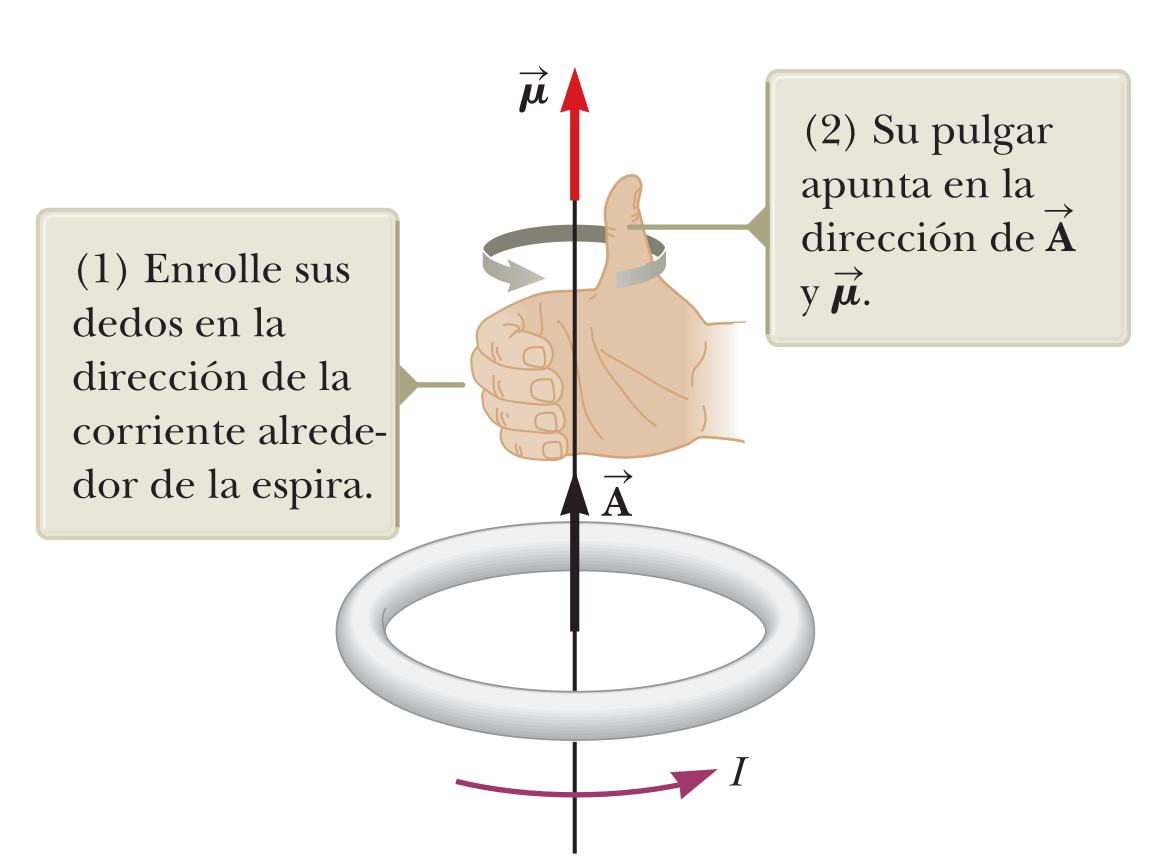
\includegraphics[width=0.5\textwidth]{dipolar_magnet_moment.png}
  \caption{Regla de la mano derecha para determinar la dirección del vector \(\vec{A}\) y el momento dipolar magnético \(\vec{\mu}\).}
  \label{fig:dipolar_magnet_moment}
\end{figure}

En base al momento dipolar magnético, se puede escribir una expresión de torque (\(\vec{\tau}\)) que experimenta un solenoide de \(N\) vueltas en presencia de un campo magnético externo (\(\vec{B}\)): 
\[
  \vec{\tau} = \vec{\mu} \times \vec{B}
\]

Si el momento magnético \(\vec{\mu}\) es paralelo al campo \(\vec{B}\), no hay momento de torsión (\(\tau = 0\)). Si \(\vec{\mu}\) es perpendicular a \(\vec{B}\), el momento de torsión es máximo. El torque tiende a alinear \(\vec{\mu}\) con \(\vec{B}\).

\begin{figure}[ht]
  \centering
  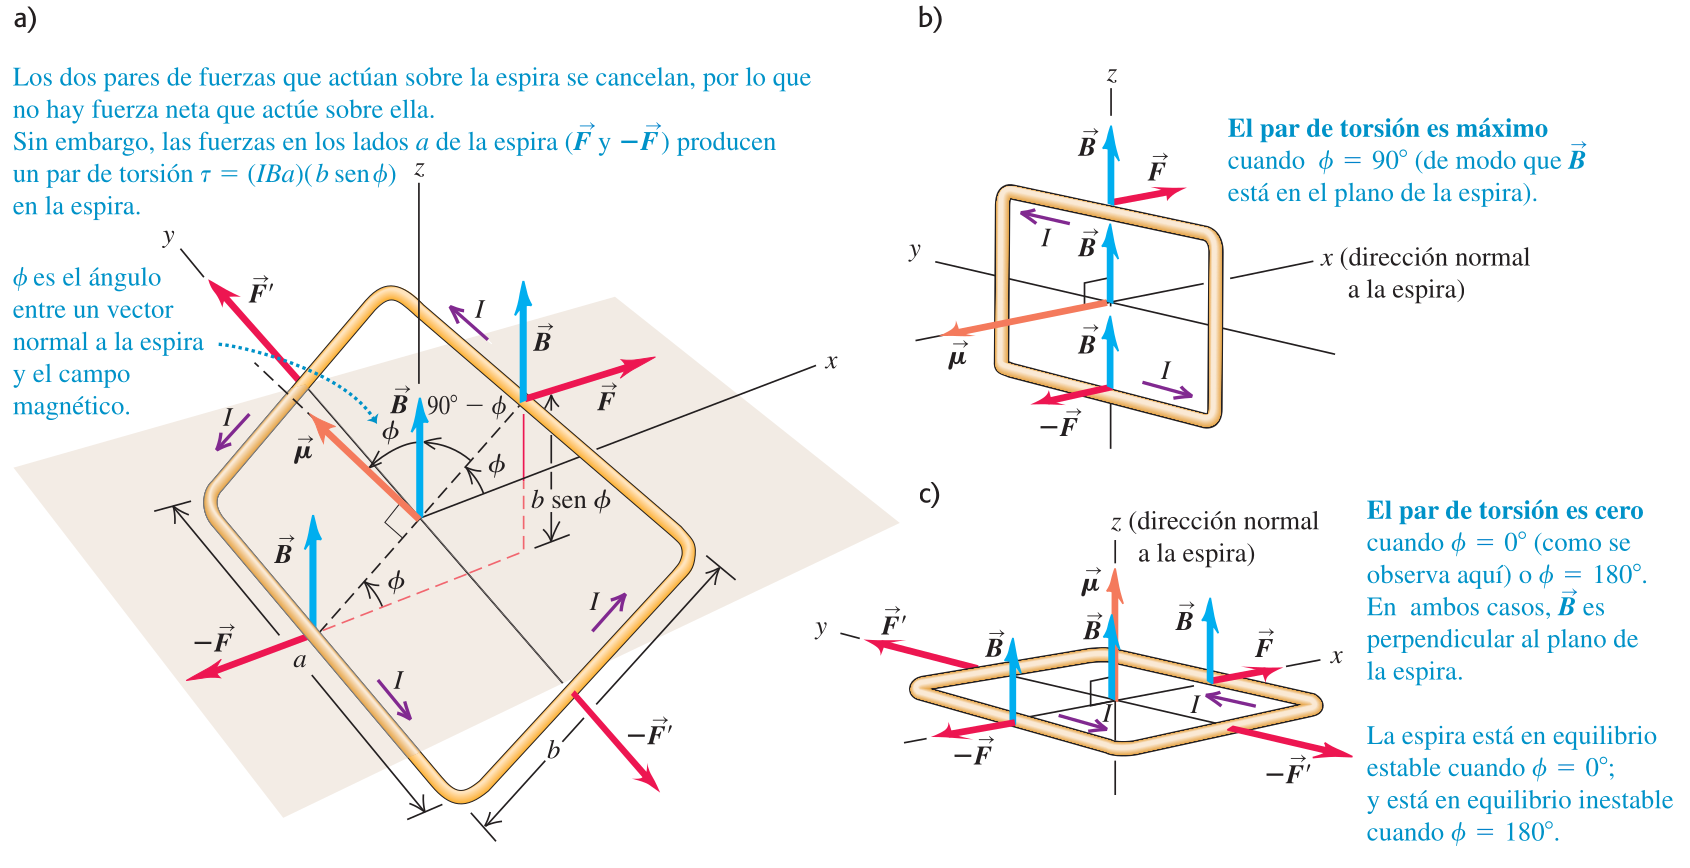
\includegraphics[width=1\textwidth]{par.png}
  \caption{Cálculo del par de torsión sobre una espira que conduce corriente en un campo magnético uniforme.}
\end{figure}

\begin{tcolorbox}[myconclusion]
  El momento magnético mide cuán magnético es un cuerpo, en el mismo sentido que el momento angular mide cuán rotacional es, y el momento lineal cuán translacional.
\end{tcolorbox}

Cuando un sistema con momento magnético \(\vec{\mu}\) se coloca en un campo magnético externo \(\vec{B}\), experimenta:
\begin{itemize}
  \item \textbf{Un torque}: \(\vec{\tau}=\vec{\mu}\times\vec{B}\) que lo alinea con el campo,
  \item \textbf{Una energía potencial}: \(U=-\vec{\mu}\cdot\vec{B}\), mínima cuando \(\vec{\mu}\) y \(\vec{B}\) están alineados.
\end{itemize}
Esto explica fenómenos como la orientación de las agujas magnéticas, el paramagnetismo, y técnicas como la resonancia magnética nuclear (RMN).

\begin{tcolorbox}[mydanger]
  \textbf{CUIDADO}: Una partícula cargada que se mueve \textbf{en línea recta} a \textit{velocidad constante} \textbf{no tiene momento magnético} (aunque sí genera un campo magnético). El momento magnético aparece solo cuando hay \textbf{movimiento cerrado o rotacional}, como una espira de corriente o una órbita de una partícula. Cuanto mayor es el momento magnético, más fuertemente responde el sistema ante un campo magnético externo, tanto en torque como en energía potencial.
\end{tcolorbox}

Puede ampliar los contenidos de torque magnético en \href{https://openstax.org/books/f%C3%ADsica-universitaria-volumen-2/pages/11-5-fuerza-y-torque-en-un-bucle-de-corriente}{OpenStax} \cite{openstax}.

\begin{tcolorbox}[interesting_data, title=Dato curioso]
  Una aplicación médica importante del par de torsión sobre un dipolo magnético son las imágenes de resonancia magnética (IRM). Se coloca a un paciente en un campo magnético de aproximadamente \(1.5 \si{\tesla}\), lo cual es \(10^4\) veces más intenso que el campo de la Tierra. El núcleo de cada átomo de hidrógeno en el tejido que se desea observar tiene un momento dipolar magnético, que experimenta un par de torsión que lo alinea con el campo aplicado. Después se ilumina el tejido con ondas de radio de la frecuencia correcta para apenas sacar a estos momentos magnéticos de su alineación. El grado en que estas ondas de radio son absorbidas por el tejido es proporcional a la cantidad de hidrógeno presente. De ahí que un tejido suave rico en hidrógeno se vea muy distinto de un hueso con poco hidrógeno, lo cual hace que la IRM sea ideal para analizar detalles de tejidos suaves que no se verían en las imágenes de rayos x  
\end{tcolorbox}

\subsection{Fuentes de campos magnéticos}

Anteriormente probablemente haya visto que partículas con masa generan un campo gravitatorio y pueden interactuar con otros campos gravitatorios. También que cargas eléctricas generan un campo eléctrico y pueden interactuar con otros campos eléctricos. Para las cargas en movimiento no es la excepción, tal y como las otras interacciones, las cargas en movimiento interactúan con campos magnéticos y generan campos magnéticos.

Antes de continuar es importante aclarar un detalle importante en la analogía de arriba. Que un objeto con masa genere un campo gravitatorio \textbf{no} significa que los campos gravitatorios interactuen entre sí. Lo mismo para los campos eléctricos y magnéticos. La interacción no es campo-campo, sino más bien \textit{objeto-campo}. En el caso del campo magnético la interacción ocurre entre una carga en movimiento y un campo magnético, o entre una corriente y un campo magnético.

\subsubsection{Campo magnético de una carga en movimiento}

Para poder explicarlo veamos la figura \ref{fig:lineas_de_campo_magnético_de_la_carga_puntual}. En esta figura se muestran las líneas de campo magnético generadas por una carga puntual que se mueve con velocidad constante.

\begin{figure}[ht]
  \centering
  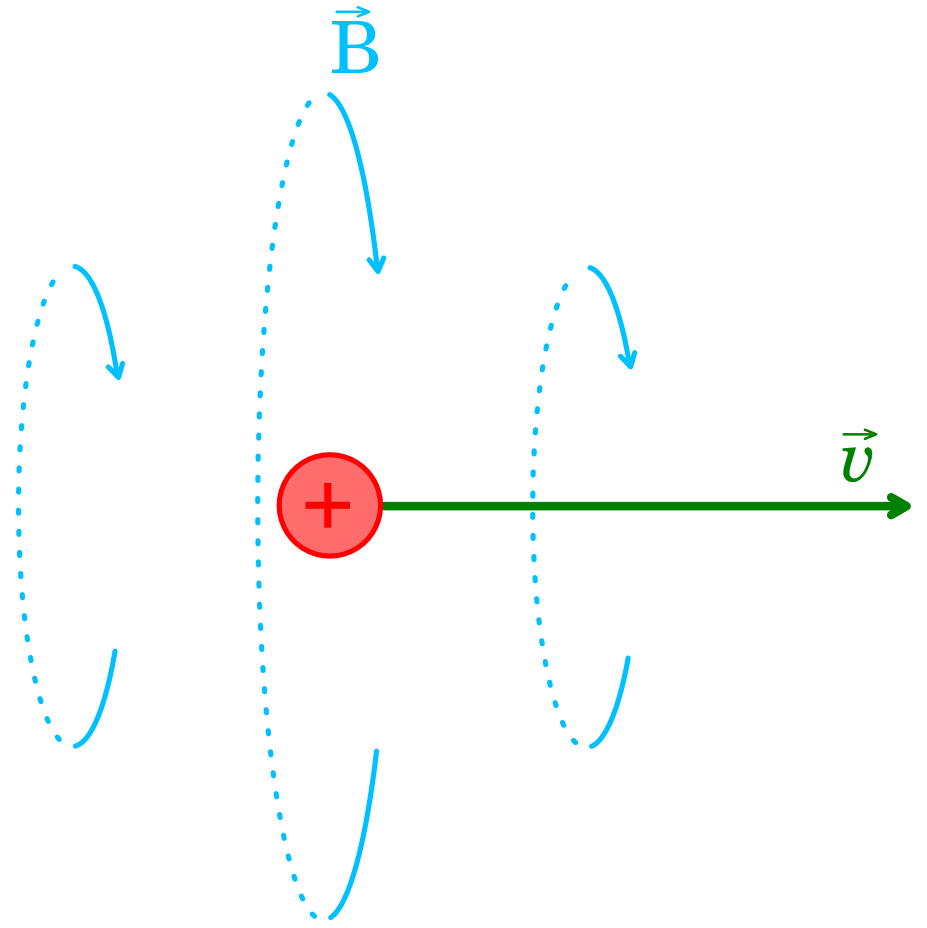
\includegraphics[width=0.3\textwidth]{squematic_charge_magnetic_field.png}
  \caption{Líneas de campo magnético de la carga puntual.}
  \label{fig:lineas_de_campo_magnético_de_la_carga_puntual}
\end{figure}

El campo magnético \(\vec{B}\) generado por la carga puntual \(q\) que se mueve con velocidad constante \(\vec{v}\) en \textbf{un punto del espacio} \(\vec{r}\) está dado por:

\begin{equation}
  \vec{B} = \frac{\mu_0}{4\pi} \frac{q \, \vec{v} \times \hat{r}}{r^2}
  \label{eq:campo_magnético_de_una_carga_puntual}
\end{equation}
donde:
\begin{itemize}
  \item \(\mu_0 = 4 \pi \times 10^{-7} \, \frac{\si{\newton}}{\si{\ampere\squared}}\) es la permeabilidad del vacío,
  \item \(\vec{r}\) es el vector que apunta desde la posición de la carga al punto donde se evalúa el campo,
  \item \(r = |\vec{r}|\) es la magnitud del vector \(\vec{r}\),
  \item \(\hat{r} = \frac{\vec{r}}{r}\) es el vector unitario en la dirección de \(\vec{r}\).
\end{itemize}

\begin{wrapfigure}{r}{0.3\textwidth}
  \centering
  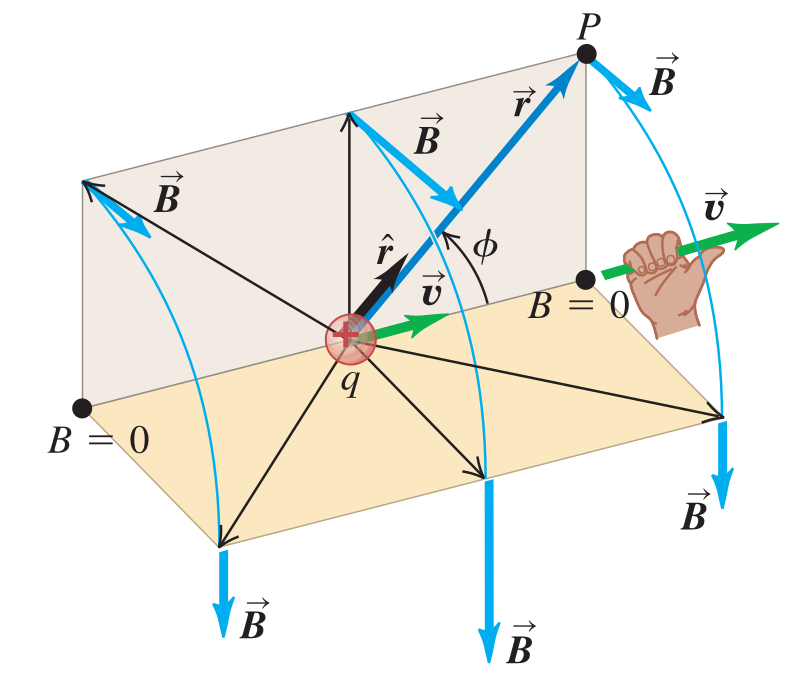
\includegraphics[width=\linewidth]{magnetic_field_of_a_point_charge.png}
  \caption{Campo magnético de una carga puntual.}
  \label{fig:campo_magnético_de_una_carga_puntual}
\end{wrapfigure}
La forma del campo magnético generado por \(q\) es circular, y \(\vec{B}\) es perpendicular a \(\vec{v}\) y \(\vec{r}\). Como se muestra en la figura \ref{fig:campo_magnético_de_una_carga_puntual} el campo magnético \(\vec{B}\) decrece con la distancia al punto \(P\). Además mientras menor es el ángulo entre \(\vec{v}\) y \(\vec{r}\) menor será el campo magnético \(\vec{B}\), y en el caso particular de \(\theta = 0^\circ\) el campo magnético \(\vec{B}\) será cero. 

Este campo magnético es el responsable de que las cargas en movimiento experimenten una fuerza magnética \(\vec{F}_B = q\vec{v} \times \vec{B}\).

Es importante recordar que \textbf{las líneas de campo magnético siempre son cerradas}. Esto lo vimos en la sección \ref{sec:flujo_magnético}, si encerramos un imán en una superficie Gaussiana, todas las líneas de campo magnético que salen, vuelven a entrar. Esto resulta en un flujo nulo.

\begin{tcolorbox}[myconclusion]
  El campo magnético total generado por varias cargas en movimiento es la suma vectorial de los campos generados por las cargas individuales.
\end{tcolorbox}

Con esto en mente, podemos encontrar el campo magnético generado por un diferencial de carga. De la sección \ref{sec:movimiento_de_cargas} sabemos que para un pedacito de segmento de longitud \(dl\) la carga es:
\[
dq = nqA\, dl
\]

De la ecuación \ref{eq:campo_magnético_de_una_carga_puntual} podemos aplicar la definición geométrica del producto vectorial, y reemplazar la carga por la expresión anterior. Entonces el campo magnético \(dB\) generado por un diferencial de carga es:
\begin{align*}
  dB &= \frac{\mu_0}{4\pi} \frac{dq \, v_d \, \sin\theta}{r^2} \\
  dB &= \frac{\mu_0}{4\pi} \frac{\left(nq v_d A\right) dl}{r^2} \sin\theta \\ 
  dB &= \frac{\mu_0}{4\pi} \frac{I dl}{r^2} \sin\theta 
\end{align*}

Entonces el un diferencial de campo magnético \(d\vec{B}\) generado por una corriente \(I\) que fluye a través de un pequeño segmento \(dl\) es:
\begin{equation}
  \boxed{d\vec{B} = \frac{\mu_0}{4\pi} \frac{I \, d\vec{l} \times \hat{r}}{r^2}}
  \label{eq:campo_magnetico_de_un_diferencial_de_corriente}
\end{equation}

\subsubsection{Ley de Biot-Savart}

La fórmula \ref{eq:campo_magnético_de_una_carga_puntual} es una versión simplificada de la Ley de Biot-Savart para una carga puntual. A partir de \eqref{eq:campo_magnetico_de_un_diferencial_de_corriente} podemos obtener la Ley de Biot-Savart que establece que el campo magnético \(\vec{B}\) generado por una corriente \(I\) que fluye a través de una curva \(C\) es:

\begin{equation}
  \vec{B} = \frac{\mu_0}{4\pi} \int_C \frac{I \, \vec{dl} \times \hat{r}}{r^2},
\end{equation}
donde:
\begin{itemize}
  \item \(\mu_0 = 4 \pi \times 10^{-7} \, \frac{\si{\newton}}{\si{\ampere\squared}}\) es la permeabilidad del vacío,
  \item \(\vec{dl}\) es el vector diferencial de longitud de la curva \(C\),
  \item \(r = |\vec{r}|\) es la magnitud del vector \(\vec{r}\),
  \item \(\hat{r} = \frac{\vec{r}}{r}\) es el vector unitario en la dirección de \(\vec{r}\).
\end{itemize}

\subsubsection{Aplicación de la ley de Biot-Savart}
\label{sec:aplicacion_de_la_ley_de_biot_savart}

La ley de Biot-Savart es una ecuación general que describe el campo magnético generado por una corriente. Sin embargo, en la práctica, su aplicación puede ser compleja, especialmente cuando se trata de curvas complejas o cuando se requiere resolver integrales complejas.

En la aplicación práctica de la ley de Biot-Savart, es común simplificar la integración considerando curvas rectas o cilíndricas, lo que permite resolver integrales más simples. Incluso es posible determinar la dirección del campo magnético con la regla de la mano derecha y calcular únicamente el módulo del campo magnético. A continuación se dan los resultados de algunos de los casos más comunes.

Para un segmento largo y recto de cable el módulo del campo magnético se convierte en:
\begin{equation*}
  B = \frac{\mu_0 I}{2\pi r}
\end{equation*}
donde:
\begin{itemize}
  \item \(\mu_0 = 4 \pi \times 10^{-7}\) es la permeabilidad del vacío,
  \item \(I\) es la corriente que fluye a través del cable,
  \item \(r\) es la distancia desde el cable al punto donde se evalúa el campo magnético.
\end{itemize}

\noindent Para una espira circular de radio \(R\) el módulo del campo magnético en el centro es:
\begin{equation*}
  B = \frac{\mu_0 I}{2R}
\end{equation*}

\noindent Para un conjunto de \(N\) espiras de radio \(R\) el campo en el centro es:
\begin{equation*}
  B = \mu_0 \frac{N I}{2R}
\end{equation*}
Este resultado se refiere a \(N\) espiras circulares (o una bobina plana) de radio \(R\), todas concentradas en el mismo plano y con el mismo centro.

\subsubsection{Ley de Ampère}

Hasta el momento, el cálculo del \hl{campo magnético} generado por una corriente ha sido realizado a través de la Ley de Biot-Savart. Sin embargo, esta ley no es la única ecuación que describe el campo magnético generado por una corriente. La Ley de Ampère es una de las ecuaciones fundamentales del electromagnetismo y establece una relación entre el campo magnético \(\vec{B}\) y las corrientes eléctricas que lo generan. 

La Ley de Ampère puede parecer abstracta al principio, pero su lógica es similar a la Ley de Gauss, aunque aplicada al magnetismo. Esta ley establece una relación entre el campo magnético \(\vec{B}\) y las corrientes eléctricas que lo generan. 
\[
\oint_{\text{lazo cerrado}} \vec{B} \cdot d\vec{l} = \mu_0 \, I_{\text{enc}}
\]
donde:
\begin{itemize}
  \item \(\vec{B}\): Campo magnético.
  \item \(d\vec{l}\): Elemento infinitesimal de un camino cerrado (lazo).
  \item \(I_{\text{enc}}\): Corriente neta encerrada por el lazo.
  \item \(\mu_0\): Permeabilidad magnética del vacío (\(4\pi \times 10^{-7} \, \mathrm{T \cdot m/A}\)).
\end{itemize}

\begin{tcolorbox}[myconclusion]
\textbf{¿Sobre qué se integra?}

En la Ley de Ampère, no se integra sobre una superficie, sino sobre un camino cerrado (lazo o bucle). Este camino cerrado se llama lazo amperiano, y es análogo a la superficie gaussiana en la Ley de Gauss, pero con diferencias importantes:
\begin{itemize}
  \item Ley de Gauss: Integral sobre una superficie cerrada.
  \subitem Relaciona el flujo eléctrico (\(\oint \vec{E} \cdot d\vec{A}\)) con la carga encerrada.  
  \item Ley de Ampère: Integral sobre un camino cerrado (una línea).
  \subitem Relaciona la circulación del campo magnético (\(\oint \vec{B} \cdot d\vec{l}\)) con la corriente encerrada.  
\end{itemize}
\end{tcolorbox}

Un camino amperiano es un camino imaginario cerrado que tú defines, al igual que la superficie gaussiana. Debe elegirse estratégicamente para aprovechar la simetría del problema (por ejemplo, círculos concéntricos alrededor de un alambre recto). 

\paragraph{¿Qué representa la integral \(\oint \vec{B} \cdot d\vec{l}\)?}

La integral \(\oint \vec{B} \cdot d\vec{l}\) se llama circulación del campo magnético y representa la suma de las componentes tangenciales de \(\vec{B}\) a lo largo del lazo amperiano. En términos físicos:
\[
\oint \vec{B} \cdot d\vec{l} = \mu_0 \, I_{\text{enc}}
\]
\begin{itemize}
  \item Lado izquierdo: Circulación del campo magnético (¿cómo ``rota'' \(\vec{B}\) alrededor del lazo?).  
  \item Lado derecho: Corriente total de conducción que atraviesa la superficie encerrada por el lazo.  
\end{itemize}

\paragraph{¿Qué buscamos con la Ley de Ampère?}

El objetivo principal es calcular el \textbf{campo magnético} (\(\vec{B}\)) en situaciones con alta simetría, donde la integral \(\oint \vec{B} \cdot d\vec{l}\) se simplifica. Por ejemplo: En un alambre infinito, un solenoide, o un toroide.  

\begin{itemize}
  \item Alambre infinito recto:  
    \[
    B = \frac{\mu_0 I}{2\pi r} \quad \text{(dirección circular alrededor del alambre)}.
    \]
  \item Solenoide ideal:  
     \[
     B = \mu_0 n I \quad \text{(campo uniforme en el interior)}.
     \]
  \item Toroide:  
     \[
     B = \frac{\mu_0 N I}{2\pi r} \quad \text{(campo circular dentro del toroide)}.
     \]
\end{itemize}
Nótese que los resultados son consistentes con la Ley de Biot-Savart. Para el alambre infinito (o largo) y recto se ha obtenido el mismo resultado. Aunque usted tal vez se pregunte ¿Qué paso con el solenoide ideal? Parece que no ha dado lo mismo que el ejemplo del conjunto de espiras. Esto es porque el solenoide tiene la forma de un cilindro, como se vió en la figura \ref{fig:solenoide}. Un solenoide es una bobina alargada con \(N\) espiras distribuidas uniformemente a lo largo de una longitud \(L\). El ejemplo de las espiras en la sección \ref{sec:aplicacion_de_la_ley_de_biot_savart} es un conjunto de espiras que no tiene forma de cilindro, sinó que están todas en el mismo plano.

\paragraph{Ejemplo práctico: Cálculo del campo magnético en un solenoide}

Consideremos un solenoide de \(N\) vueltas, longitud \(L\), y corriente \(I\):

\textbf{Definimos el lazo amperiano}: Rectángulo que abarca parte del solenoide.

\textbf{Aplicación de Ampère}: 
\[
  \oint \vec{B} \cdot d\vec{l} = B \cdot L_{\text{interior}} = \mu_0 n I L_{\text{interior}},
\]
donde \(n = N/L\) (vueltas por unidad de longitud).  

\textbf{Resultado}: 
\[
  B = \mu_0 n I.
\]